\documentclass[12pt]{article}

\usepackage{units}
\usepackage{graphicx}

\setlength{\oddsidemargin}{0in}
\setlength{\evensidemargin}{0in}
\setlength{\textwidth}{6.5in}
\setlength{\topmargin}{-.3in}
\setlength{\textheight}{9in}
\pagestyle{empty}

\graphicspath{{images/}}

\usepackage{cleveref}
%\crefformat{equation}{equation (#2#1#3)} % this is to remove the space...
\Crefname{equation}{Equation}{Equations}
\crefname{equation}{Eq.}{Equations}

\crefformat{section}{\S#2#1#3}
\crefformat{subsection}{\S#2#1#3}
%\crefname{subsection}{\S}{\S}
\Crefname{section}{Section}{Sections}
\Crefname{subsection}{Section}{Sections}

\crefname{figure}{Fig.}{Figures}
\Crefname{figure}{Figure}{Figures}

%----------------------------------------------------------------------------------------
%	TITLE SECTION
%----------------------------------------------------------------------------------------

\title{	
\normalfont \Large 
\textsc{Visualization Project: Campus Safety and Security} \\ [10pt] % Your university, school and/or department name(s)
%\horrule{0.5pt} \\[0.4cm] % Thin top horizontal rule
Mohsen Abbasi\footnote{UID: u1011952, Email: m.abbasi@utah.edu} \\ % The assignment title
Amir Biglari\footnote{UID: u0613945, Email: amir.biglari@utah.edu}\\
Waiming Tai\footnote{UID: u1008421, Email: u1008421@utah.edu}
%\horrule{0.5pt} \\[0.4cm] % Thick bottom horizontal rule
}

%\author{Mohsen Abbasi \\ Ashkan Bashardoust} % Your name

%\date{\normalsize\today} % Today's date or a custom date

\begin{document}

\maketitle
\noindent
\textbf{Introduction:}\\
Choosing an institution is a major decision for students and their families. Along with academic, financial and 
geographic considerations, the safety of campus is a vital concern. We're planning to work on "The Campus Safety and Security"\footnote{http://ope.ed.gov/campussafety} data set to create a tool which could be used to address this issue.\\ 

\noindent
\textbf{Goals:}\\
By visualizing this data set, we have a few objectives in mind:
\begin{itemize}
\item Answering basic questions such as: 1. Which states have the safest campuses across the United States? 2. Which schools are facing some specific type of criminal activities more than the others? 3. Which schools are similar considering a particular type of crime?   
\item We're interested in comparing different schools in details and finding out what types of crimes which play a more significant role in threatening the safety of schools.
\item As mentioned above, subjects such as hate crimes and violence against women are included in the data set. It will be interesting to combine this data set with other ones containing demographic information, GDP and such for different states and look for correlations between the crime rates and these attributes. 
\end{itemize}

\noindent
\textbf{Data and Preprocessing:}\\
The Campus Safety and Security data set consists of the statistics for different types of criminal activities at postsecondary institutions in the United States between 2001 and 2014. The crimes covered in the data set are categorized into criminal offenses such as theft, disciplinary actions such as drug violations, hate crimes, VAWA offenses and others.\\
Fortunately (for the sake of safety on campuses), "The Campus Safety and Security" data set is a sparse one (there are many zero values in each record). Therefore, we have to create new versions of data set by combining different records based on our needs. In addition, while the survey is conducted each year for 14 years, a lot of missing data points exist in the datt set which should be taken care of.\\


\noindent
\textbf{Visualization Design:}\\
There are three phenomenons we would like to study and visualize:
\begin{enumerate}
\item The crime statistics for different institutes in each state. Also, see how these statistics have changed over time.
\item Analyze the statistics by choosing a specific type of crime. For each type of crime, the trend for different categories of that crime over time will be shown in graphs.
\item Comparing the crime statistics between different schools. By choosing two or more schools, different types of crime would be compared.
\end{enumerate}
The following are the designs we'd like to consider:\\

\noindent	
\textbf{Crime statistics in each state:} This design would be to display the map of the United States. Here each state is colored using a gradient color map that uses saturation with respect to the crime number per students in that state. The map is broken down by states where each one is selectable. There is also a time line bar that can be adjusted to the desired year. Beside the map there would be a line chart showing the trend of the change in the number of different types of crimes in US universities in time (\cref{fig:p1-overall}). By selecting a specific type you would be able to see a bar plot showing the amount of crimes for different crime categories of that type (\cref{fig:p1-1}). By hovering over a state you can see a general information about it (\cref{fig:p1-2}). By choosing a state, line chart and the barchart beside the map would get updated with respect to that specific state. The general crime statistics would also be displayed below the map on a line chart in which each line represents a school in the selected state (\cref{fig:p1-3}) and by hovering over the lines you can see the schools names (\cref{fig:p1-4}). Also, when a line in the line chart is selected, the detail breakdown of different types of crimes would be displayed on a stack bar chart (\cref{fig:p1-5}). By selecting each chunk of the stack bar chart, you will get another stack bar chart for the categories of that crime type for the specific school (\cref{fig:p1-6}). There would be two search boxes to search any two schools and compare their crime statistics. By selecting a pair of schools and do hitting the compare button the user will get a new view which compares the school crime statistics in line charts and bar charts.
\\

\begin{figure}[tbph]
   \centering{}
	       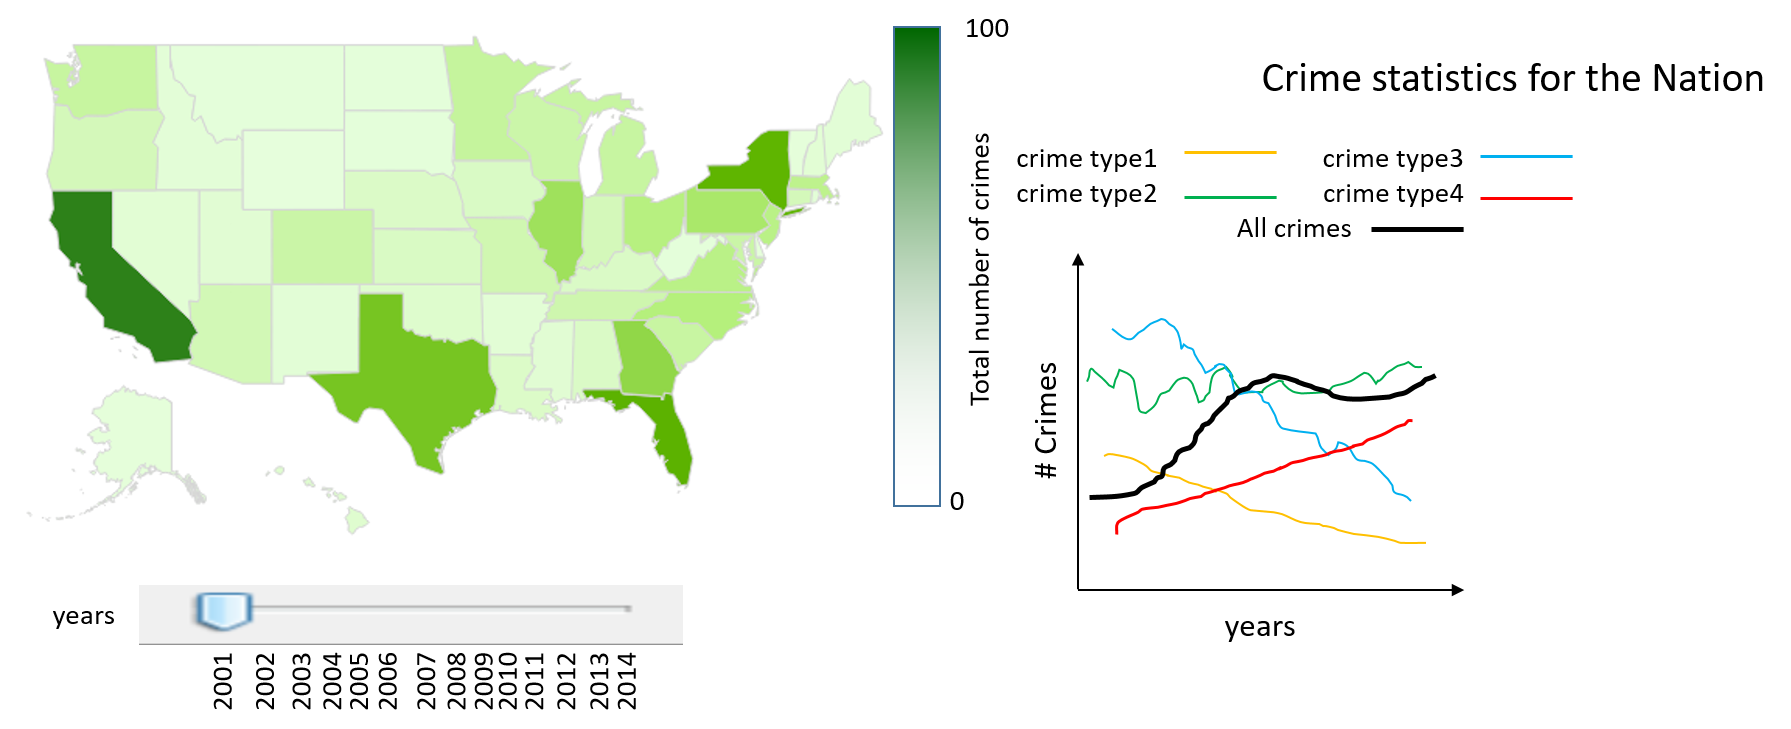
\includegraphics[width=6in]{prot1-overall}           
\caption{}
\label{fig:p1-overall}
\end{figure}

\begin{figure}[tbph]
   \centering{}
	       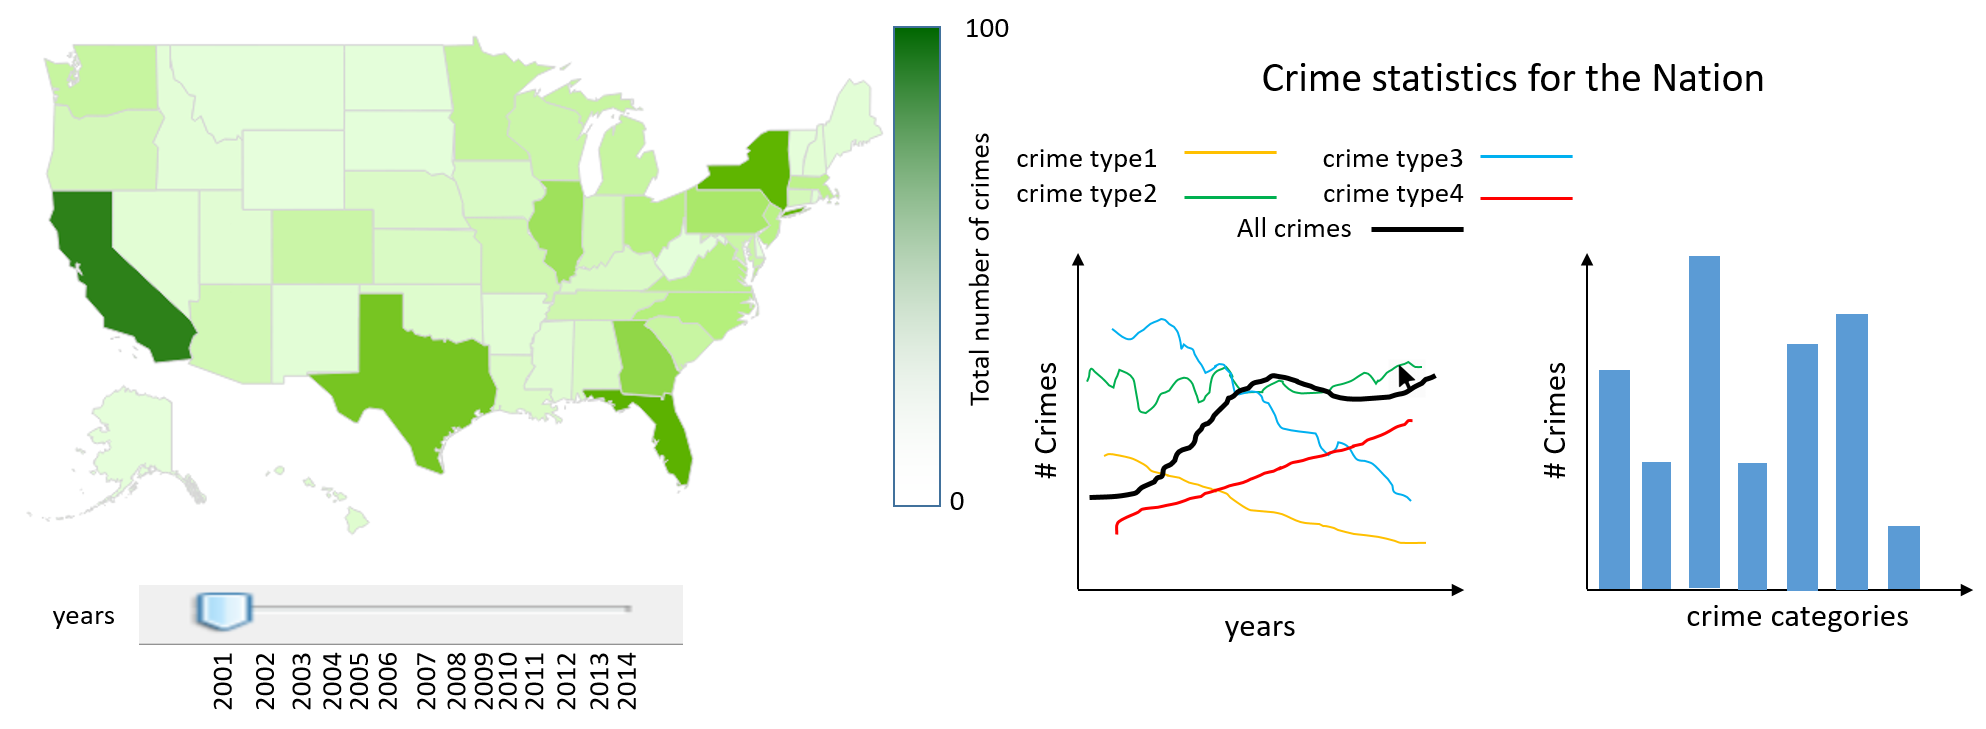
\includegraphics[width=6in]{prot1-1}           
\caption{}
\label{fig:p1-1}
\end{figure}

\begin{figure}[tbph]
   \centering{}
	       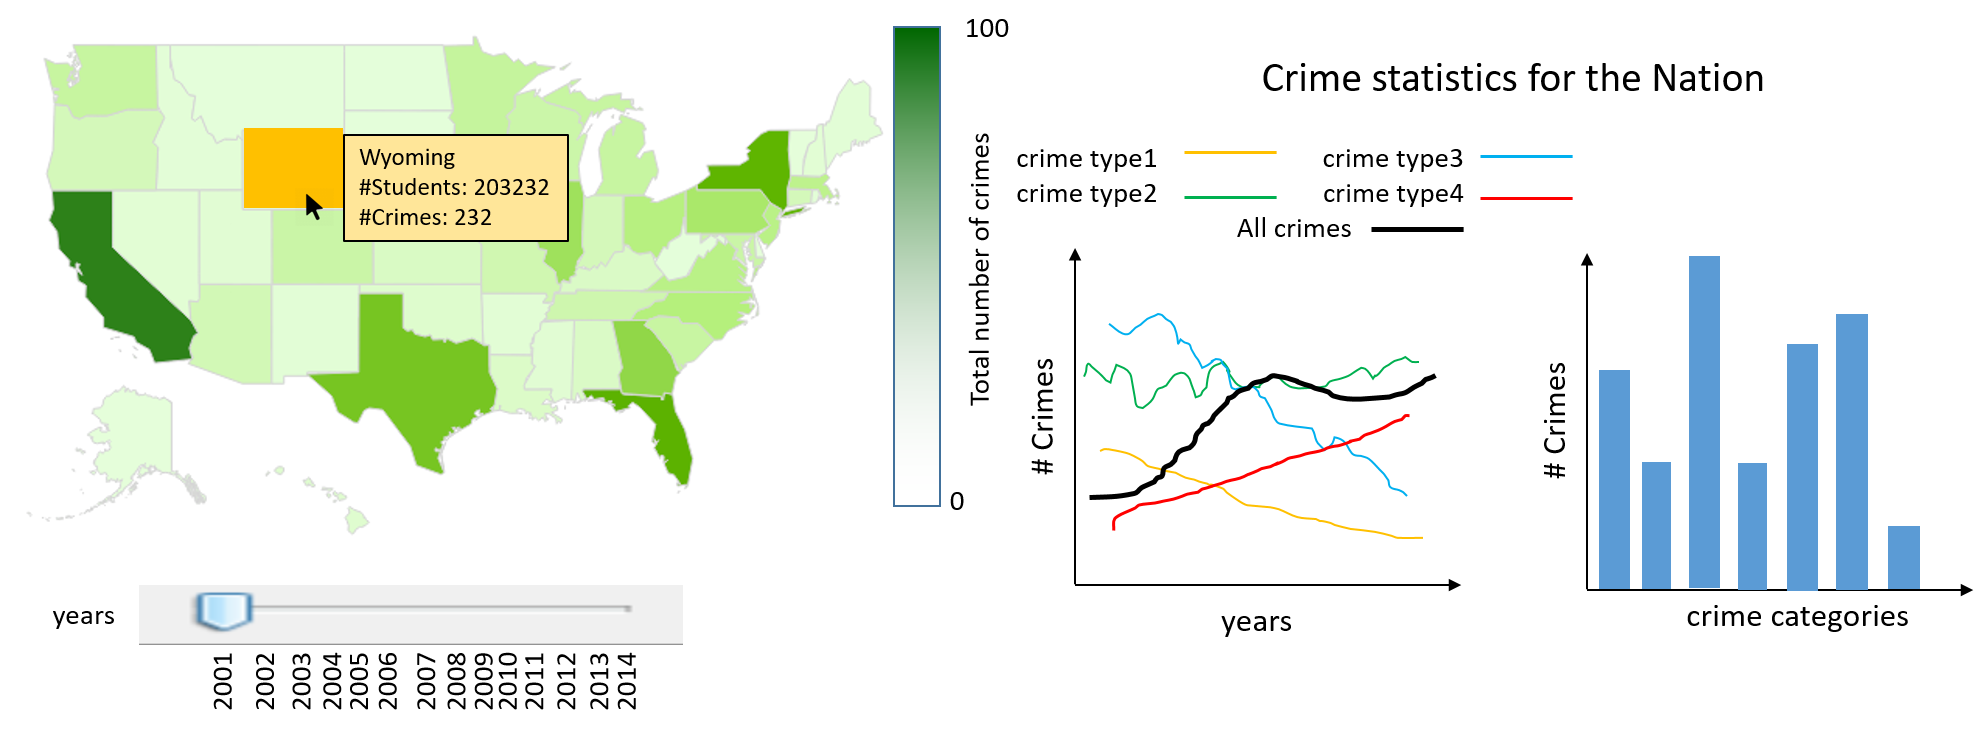
\includegraphics[width=6in]{prot1-2}           
\caption{}
\label{fig:p1-2}
\end{figure}

\begin{figure}[tbph]
   \centering{}
	       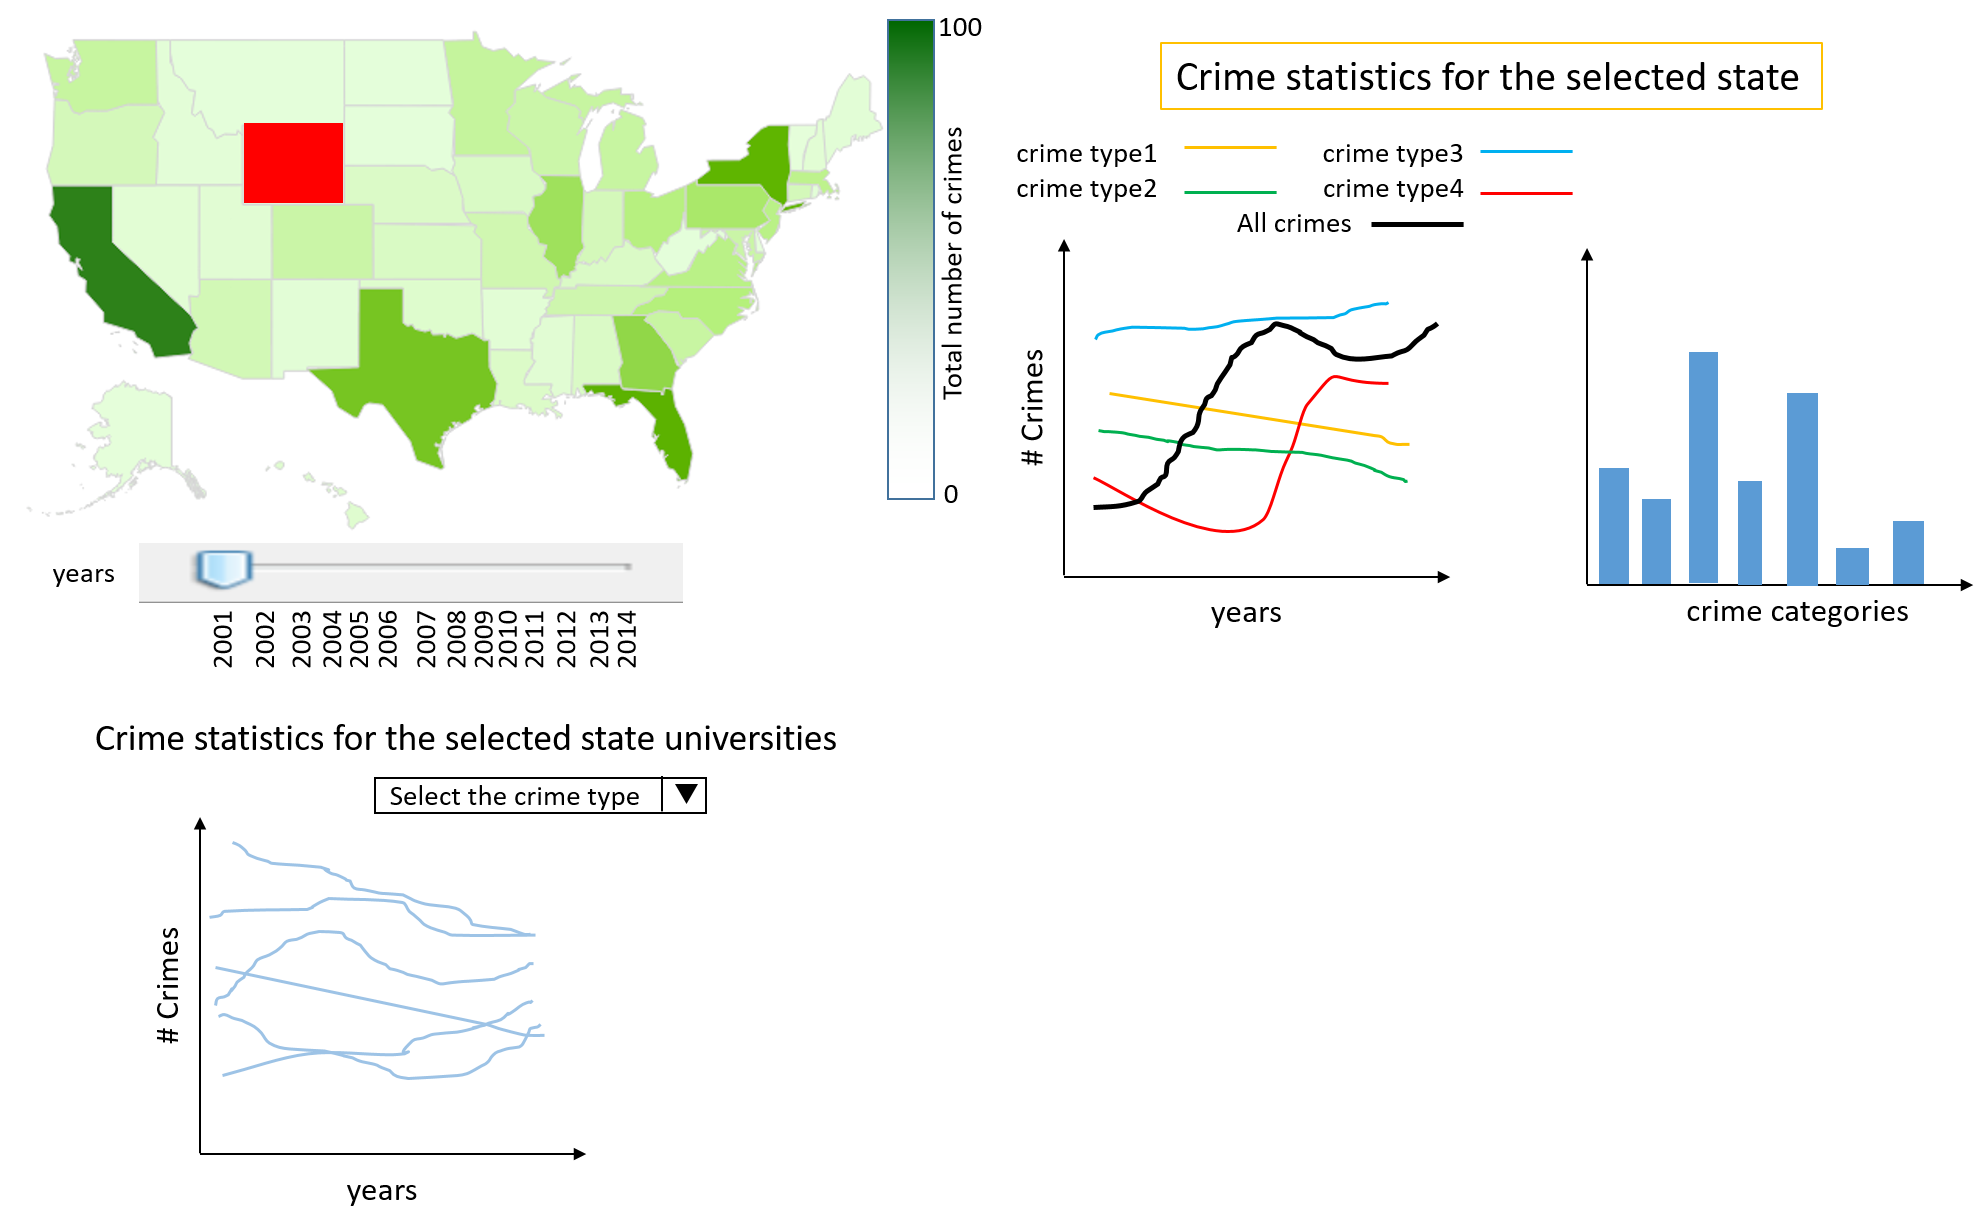
\includegraphics[width=6in]{prot1-3}           
\caption{}
\label{fig:p1-3}
\end{figure}

\begin{figure}[tbph]
   \centering{}
	       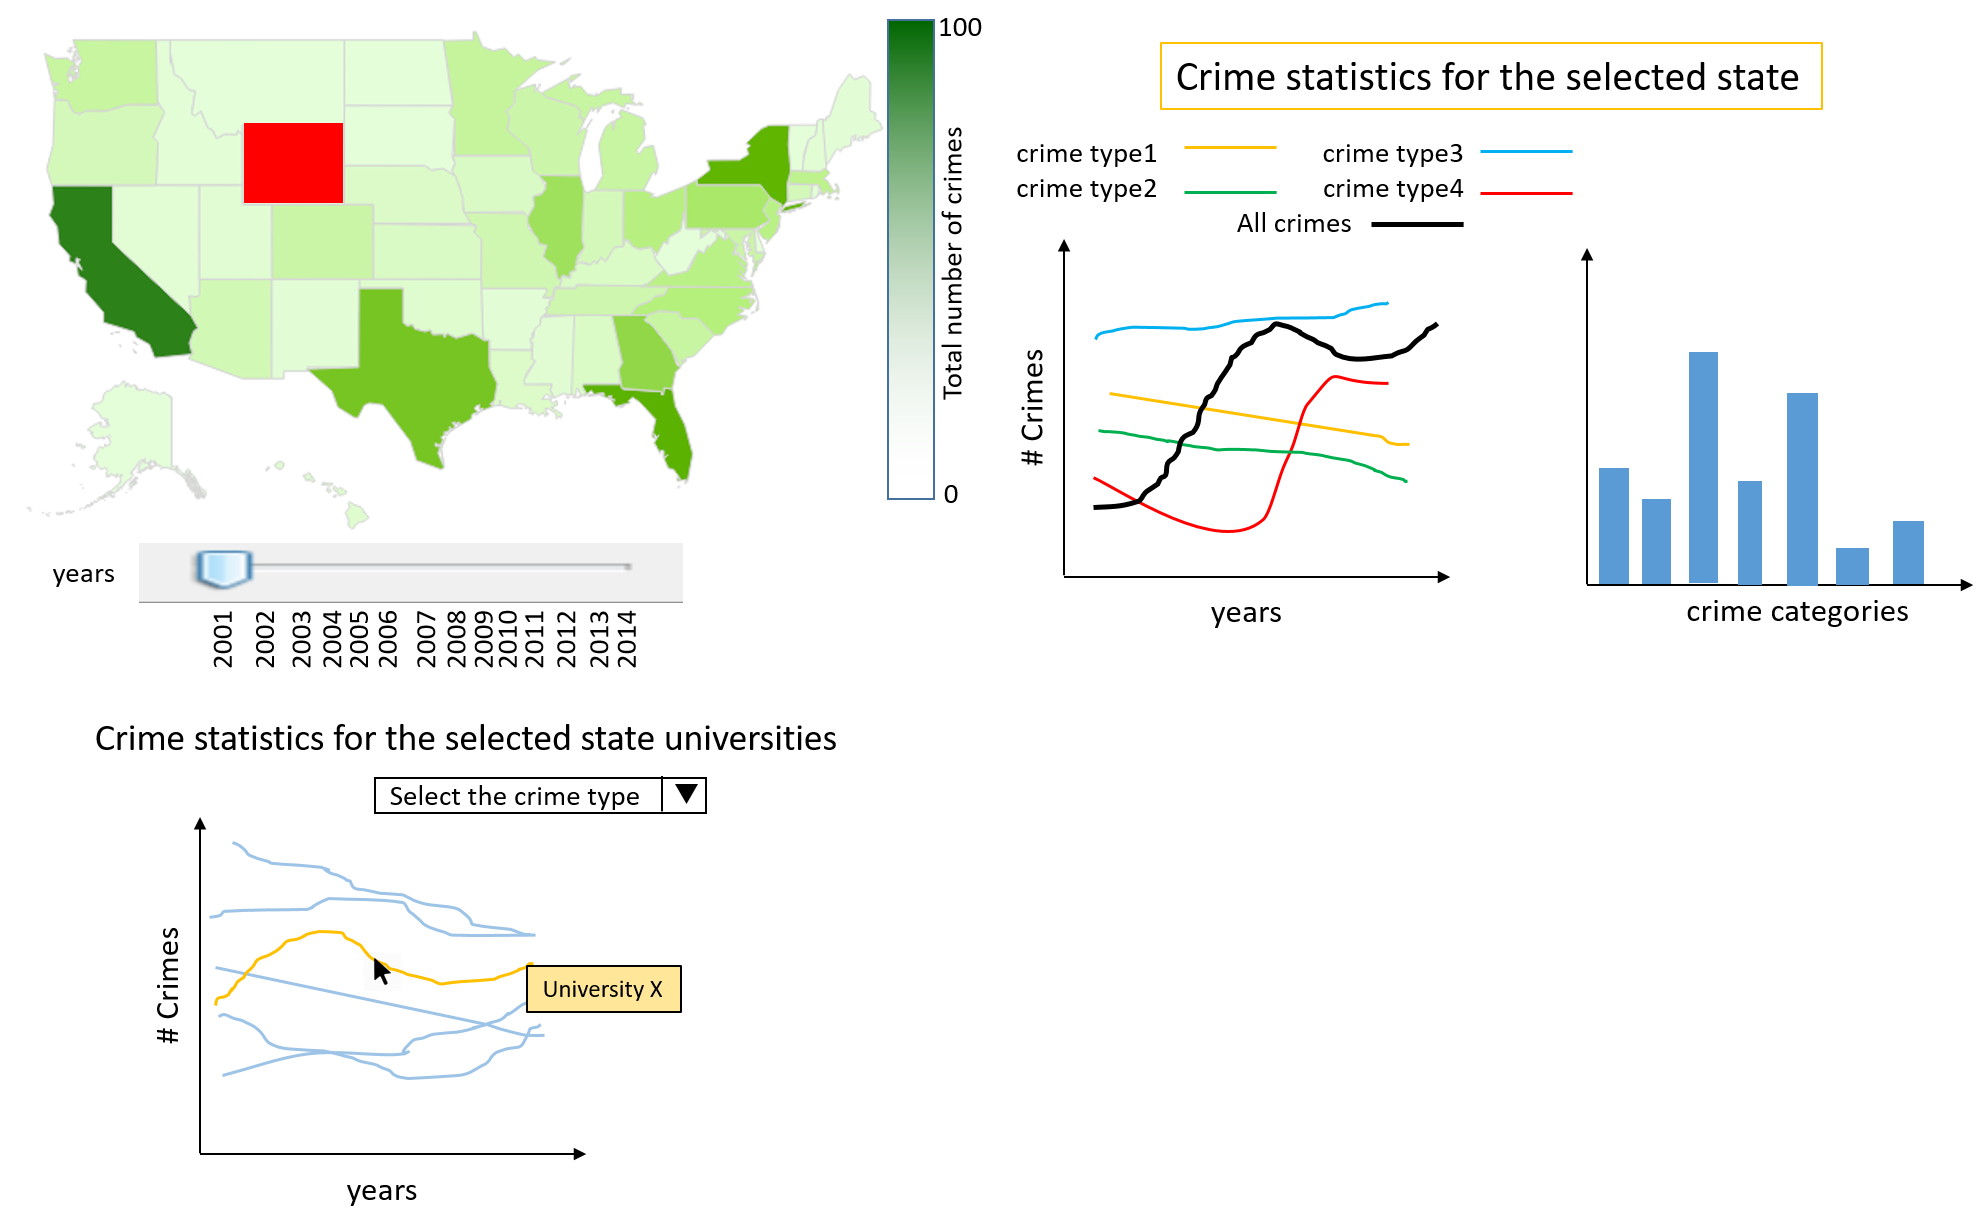
\includegraphics[width=6in]{prot1-4}           
\caption{}
\label{fig:p1-4}
\end{figure}

\begin{figure}[tbph]
   \centering{}
	       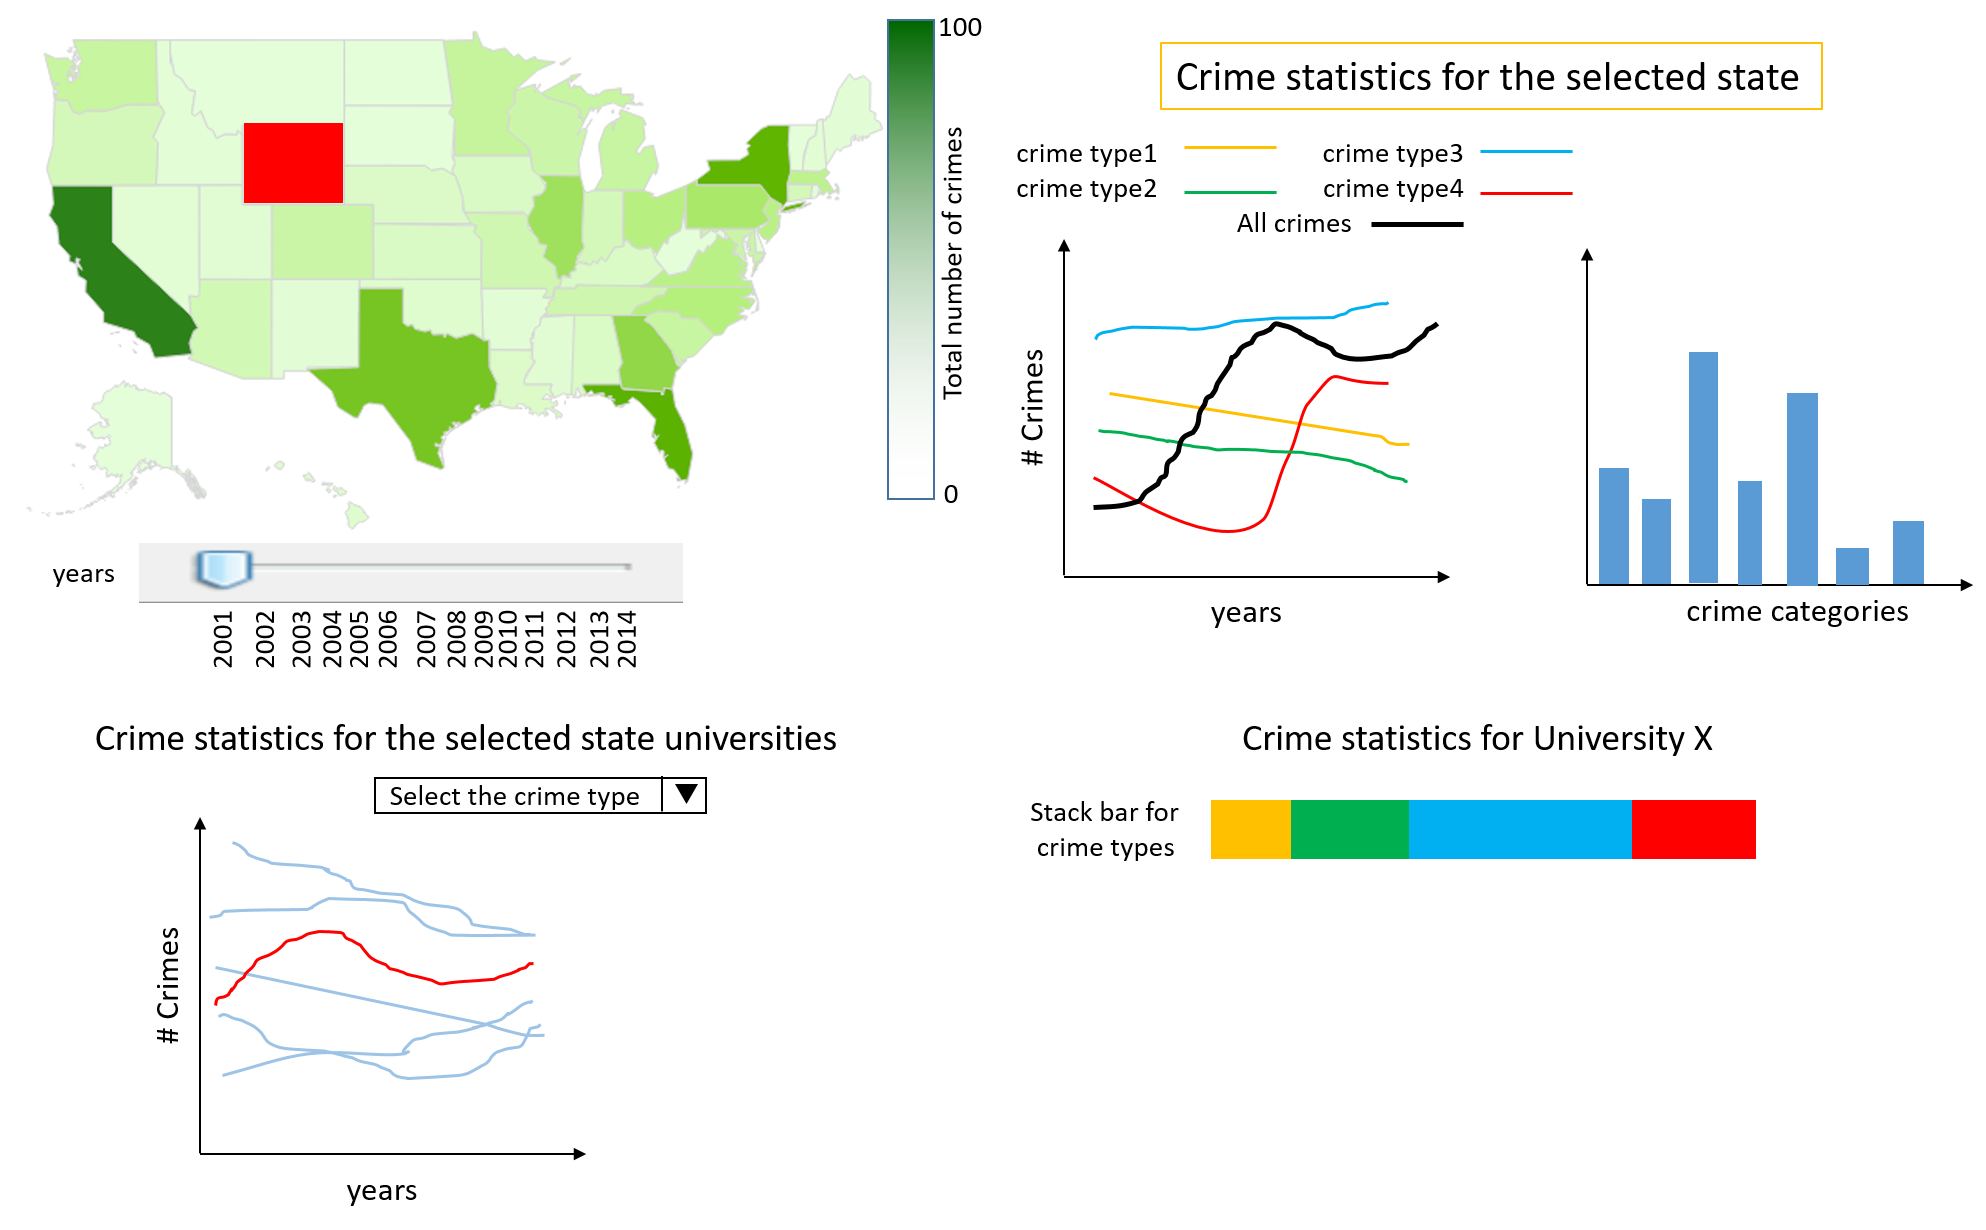
\includegraphics[width=6in]{prot1-5}           
\caption{}
\label{fig:p1-5}
\end{figure}

\begin{figure}[tbph]
   \centering{}
	       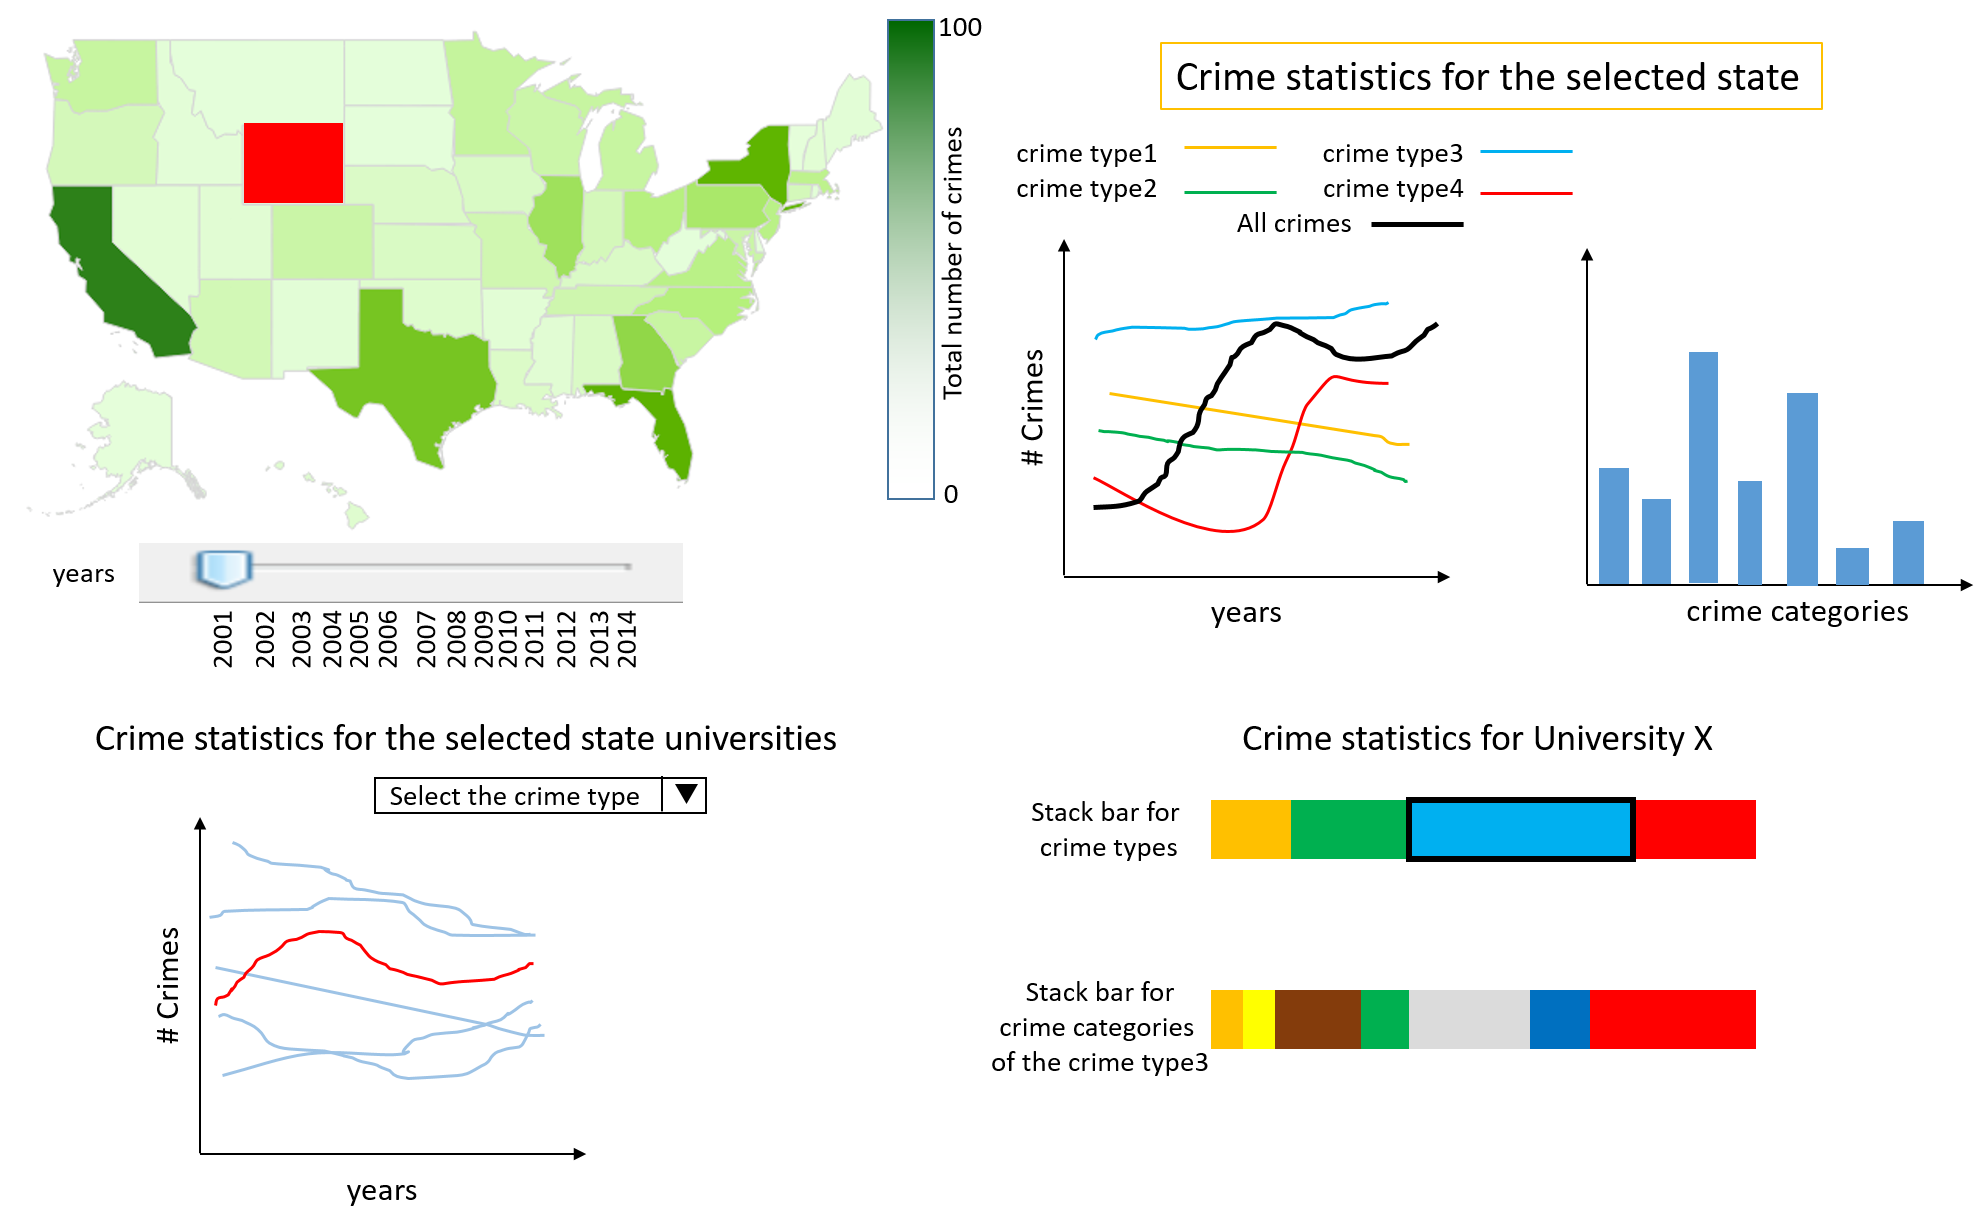
\includegraphics[width=6in]{prot1-6}           
\caption{}
\label{fig:p1-6}
\end{figure}


\noindent
\textbf{Clustering the data} This design will also have the map of the United States. This time we use a scatter plot chart to visualize the data for the whole nation or the selected states (\cref{fig:p3-1}). In this scatter plot, the x-axis represents the total number of crimes while the y-axis represents the number of students. Circles on the scatter plot represent the schools. Therefore, the ratio of the number of crimes to the number of students could be observed on the chart. These information will get updated as the slider for different years gets changed to see how these data get changed over the years. In this prototype in addition to selecting the states, you can use brushing on university circles, to update the selected university line chart and stack bar chart that we had in the first design as well (\cref{fig:p3-2,fig:p1-6}). 
\\

\begin{figure}[tbph]
   \centering{}
	       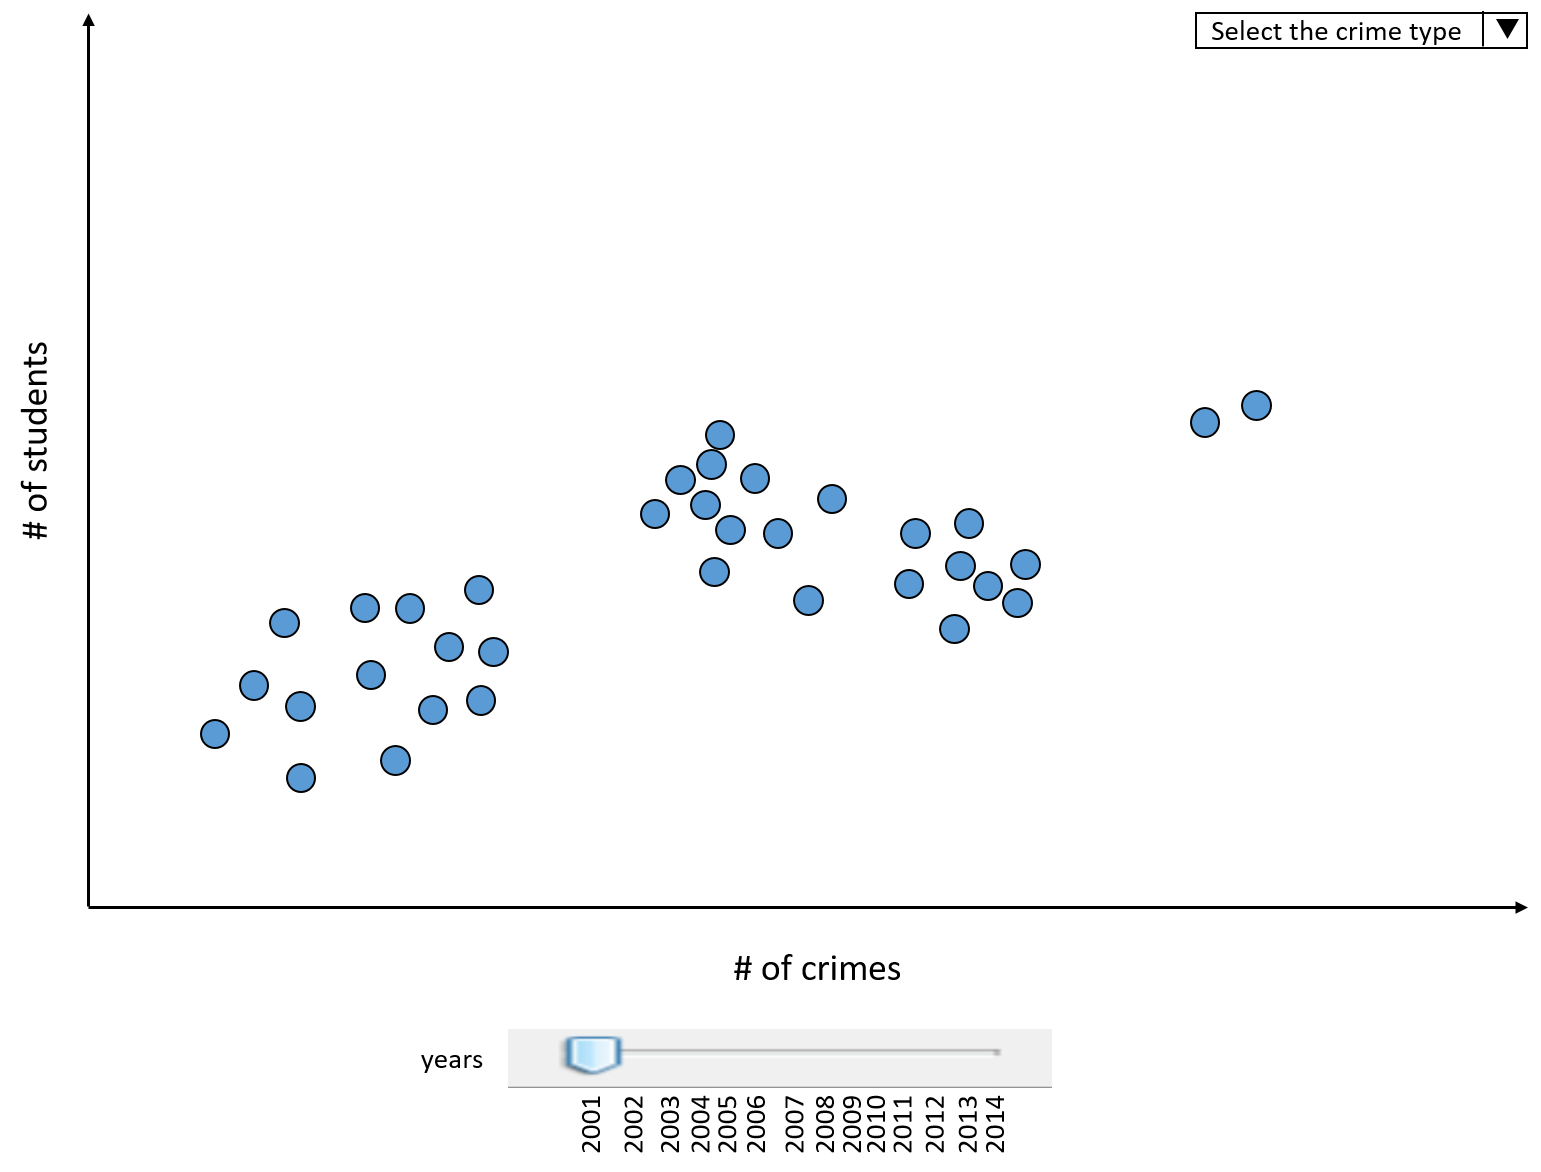
\includegraphics[width=6in]{prot3}           
\caption{}
\label{fig:p3-1}
\end{figure}

\begin{figure}[tbph]
   \centering{}
	       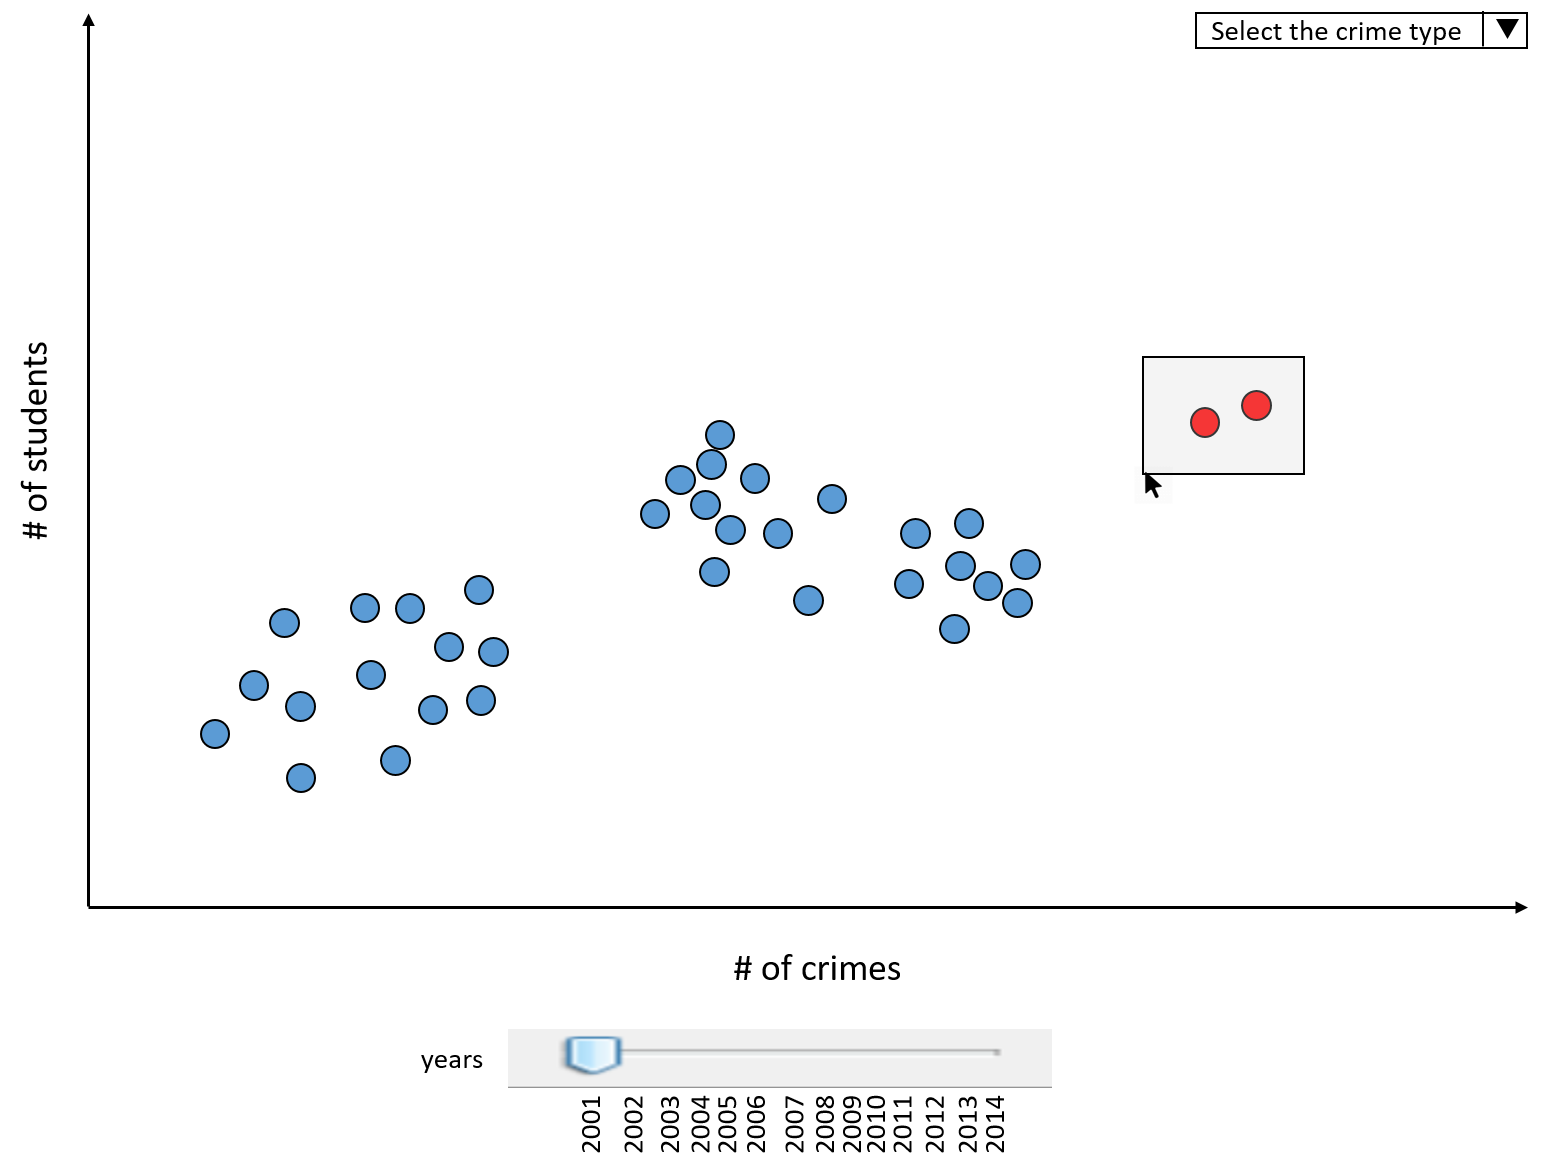
\includegraphics[width=6in]{prot3-2}           
\caption{}
\label{fig:p3-2}
\end{figure}


\noindent
\textbf{Comparing different types of crime:} In this design instead of a map we display all the universities with circles on the screen. The size of the circles are proportional to the number of the students at each school (\cref{fig:p2-overall}). They are colored using a gradient colormap that uses saturation to show the total number of the crimes at each school over the number of students. The location of the circle gives us a sense of the ratio of four different types crime compared to each other. Namely, if the circle leans on the corner representing criminal offense, the proportion of criminal offense in the corresponding school is higher. Here by hovering over a circle we can highlight it and see the name of te school bold and clear and also the exact number of crimes in that school \cref{fig:p2-1}. There would be a bruch selection to compare statistics of some desired schools in line charts (\cref{fig:p2-2}) and for a selected school on stack barcharts (\cref{fig:p2-3}).
\\

\begin{figure}[tbph]
   \centering{}
	       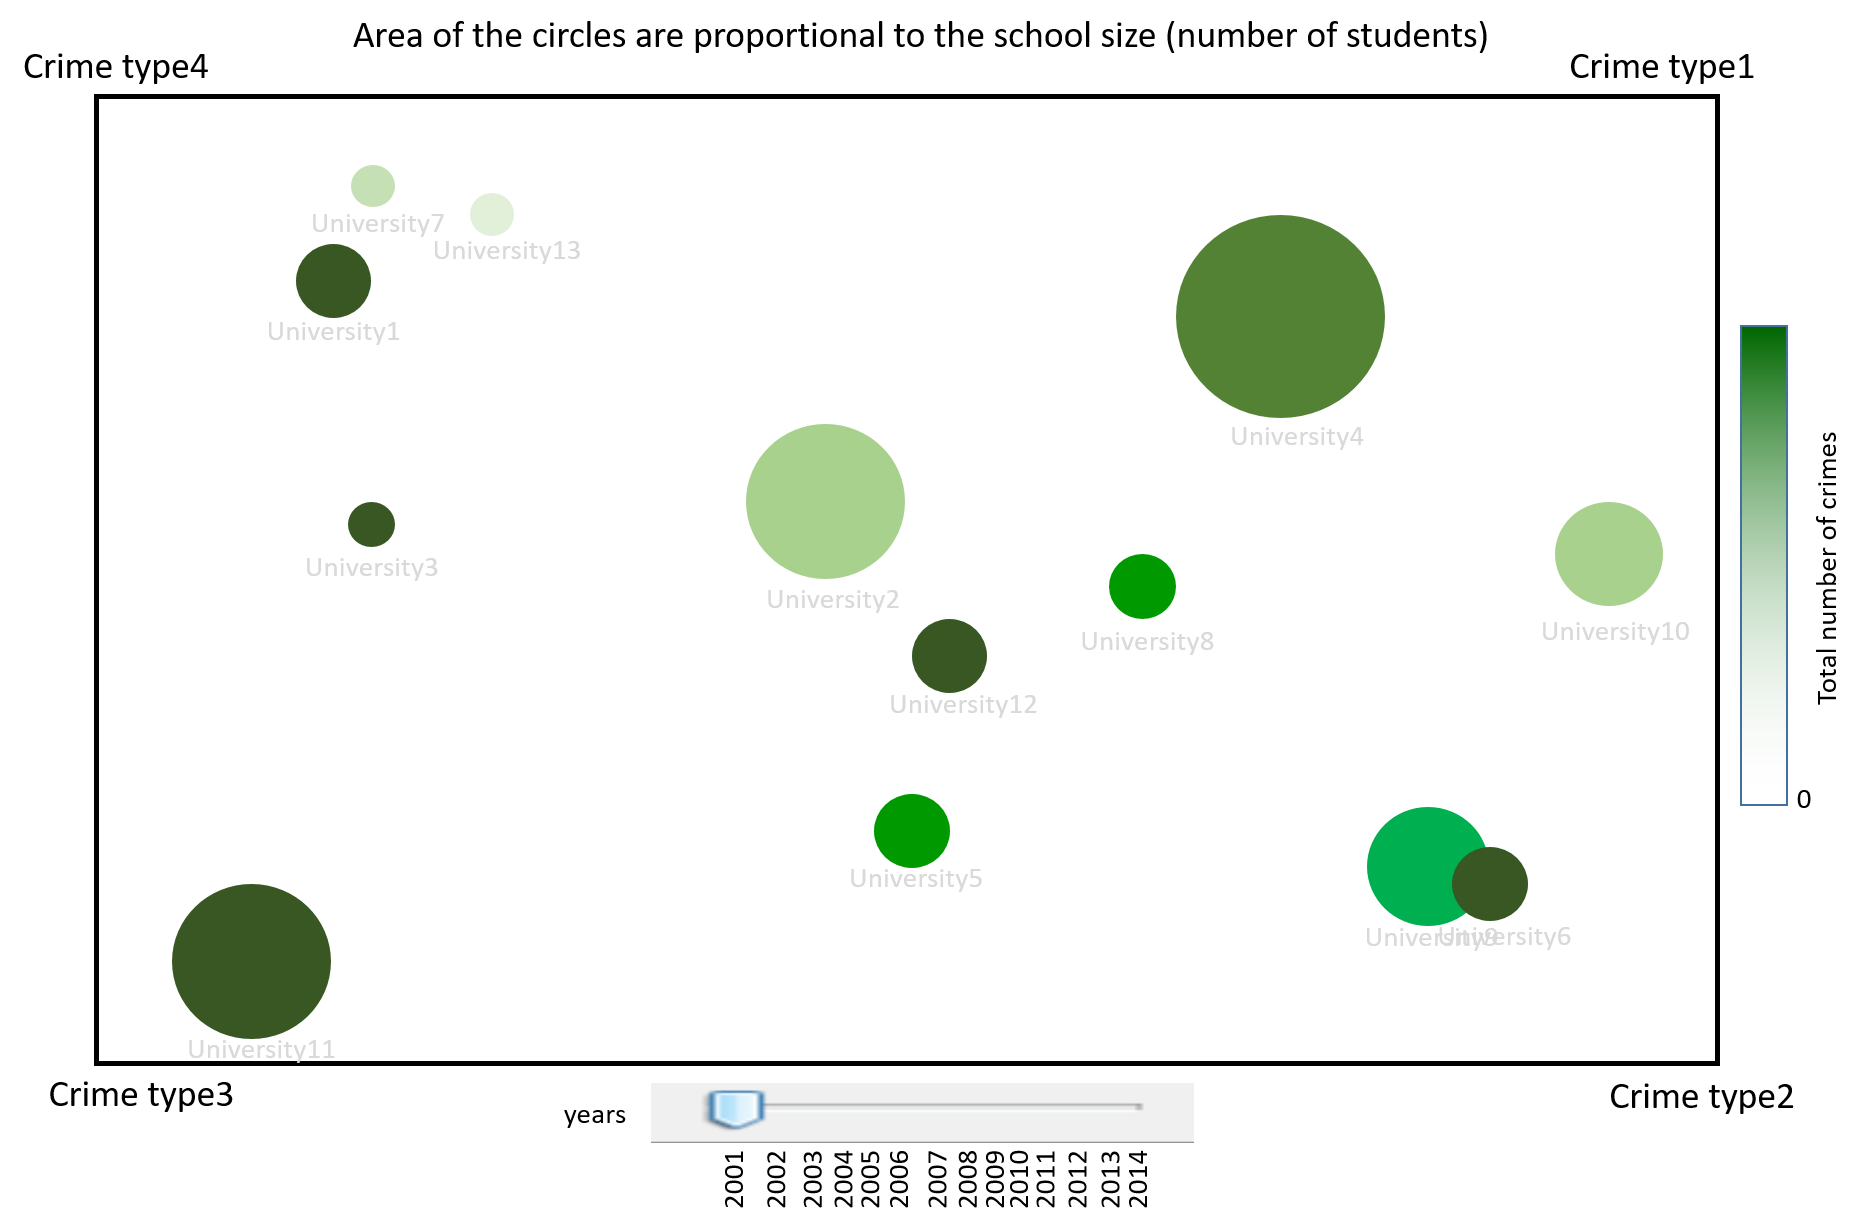
\includegraphics[width=6in]{prot2-overall}           
\caption{}
\label{fig:p2-overall}
\end{figure}

\begin{figure}[tbph]
   \centering{}
	       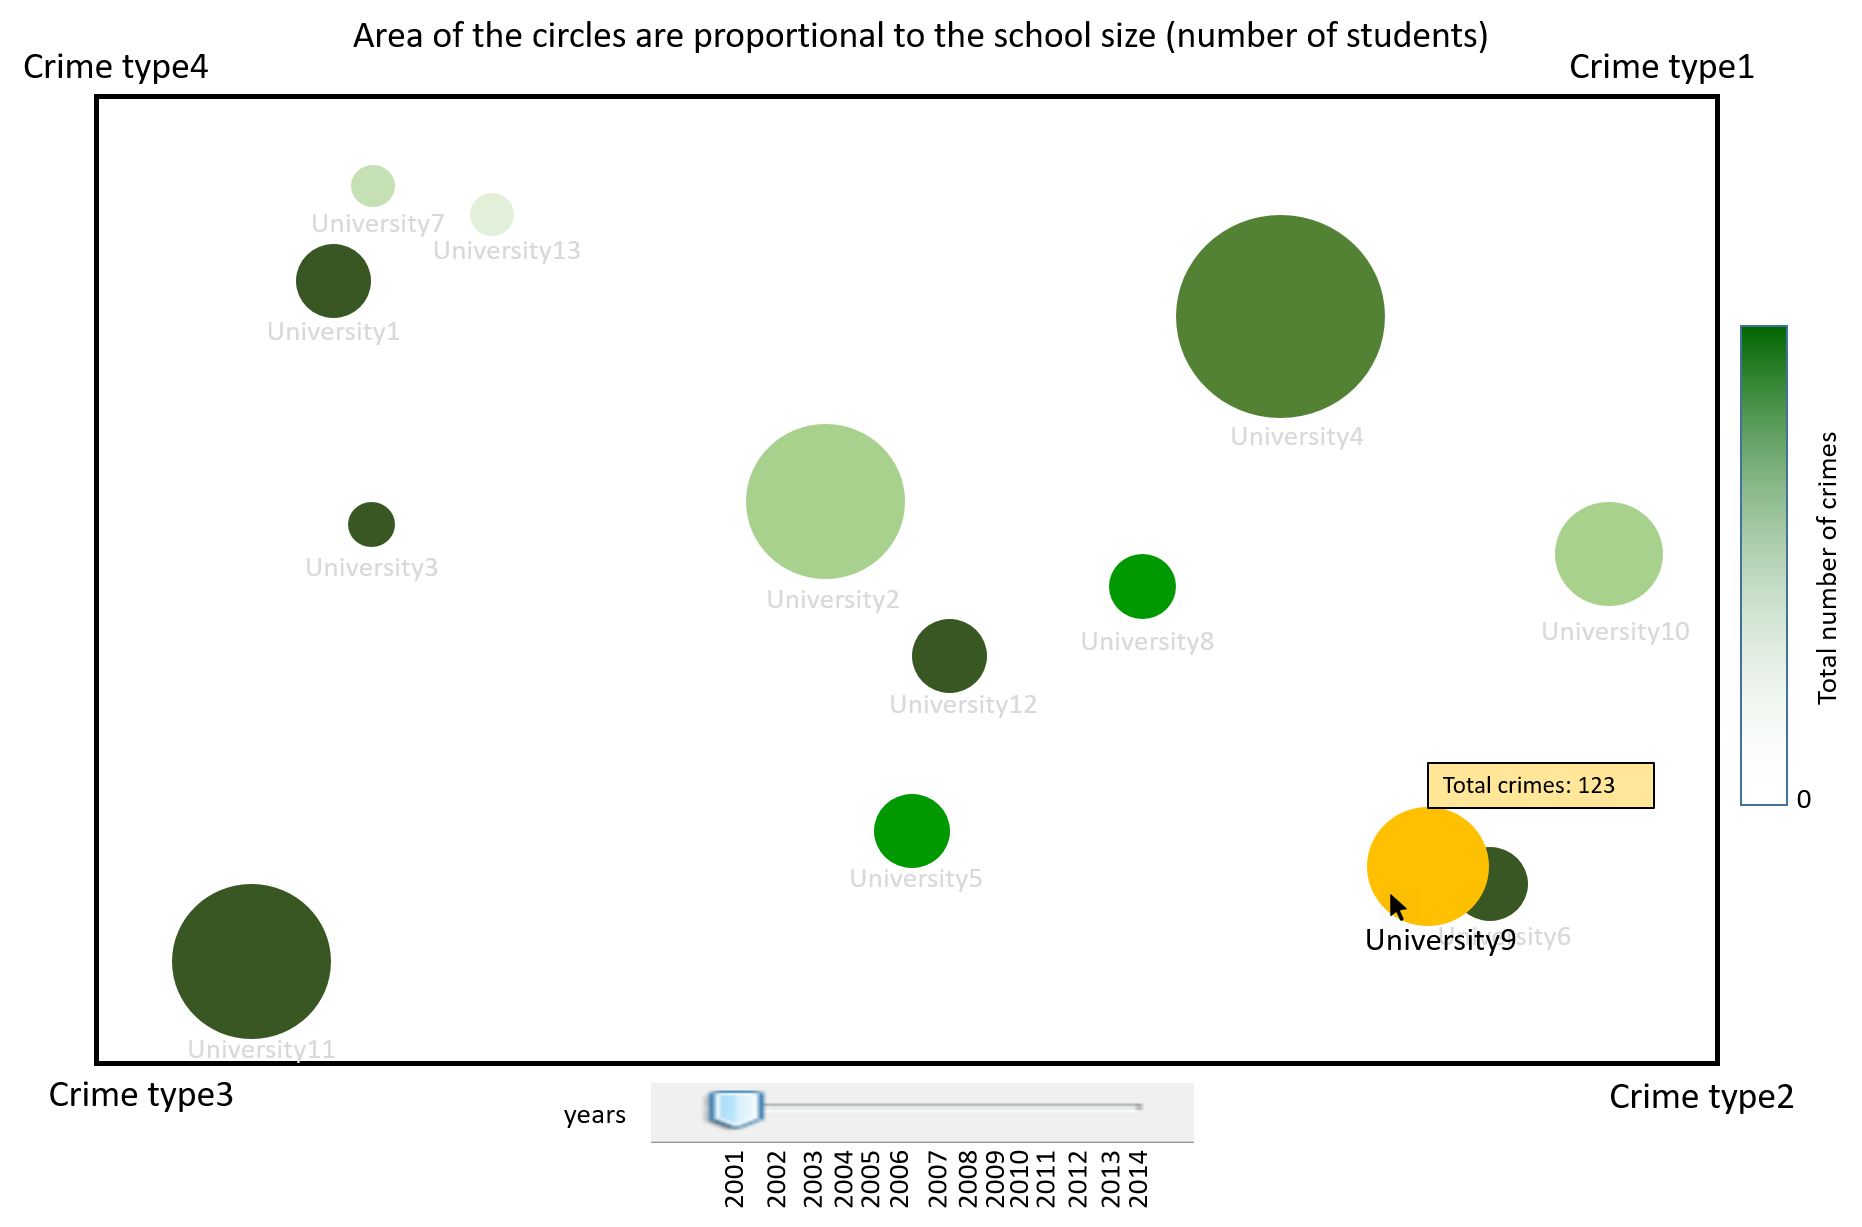
\includegraphics[width=6in]{prot2-1}           
\caption{}
\label{fig:p2-1}
\end{figure}

\begin{figure}[tbph]
   \centering{}
	       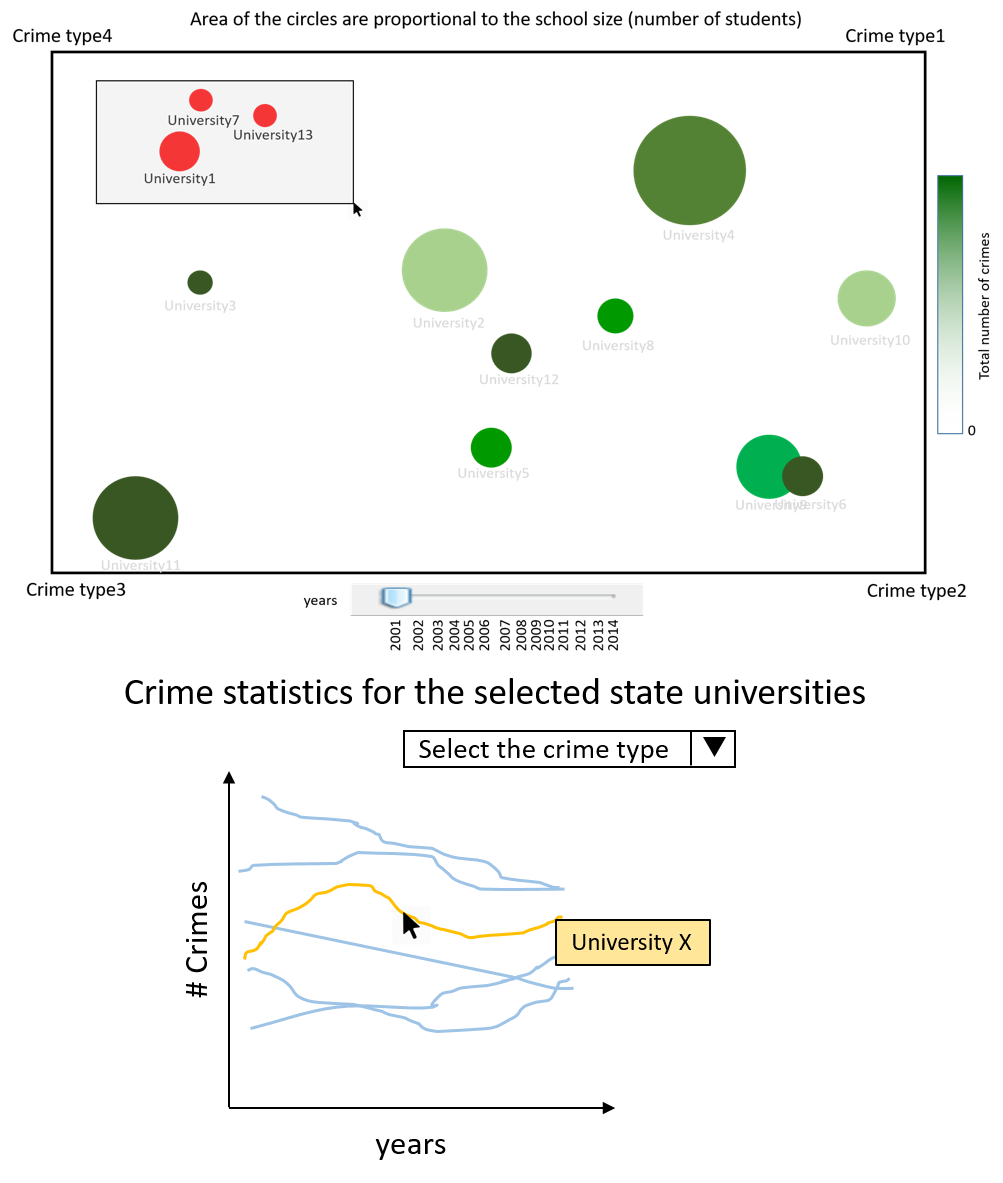
\includegraphics[width=6in]{prot2-2}           
\caption{}
\label{fig:p2-2}
\end{figure}

\begin{figure}[tbph]
   \centering{}
	       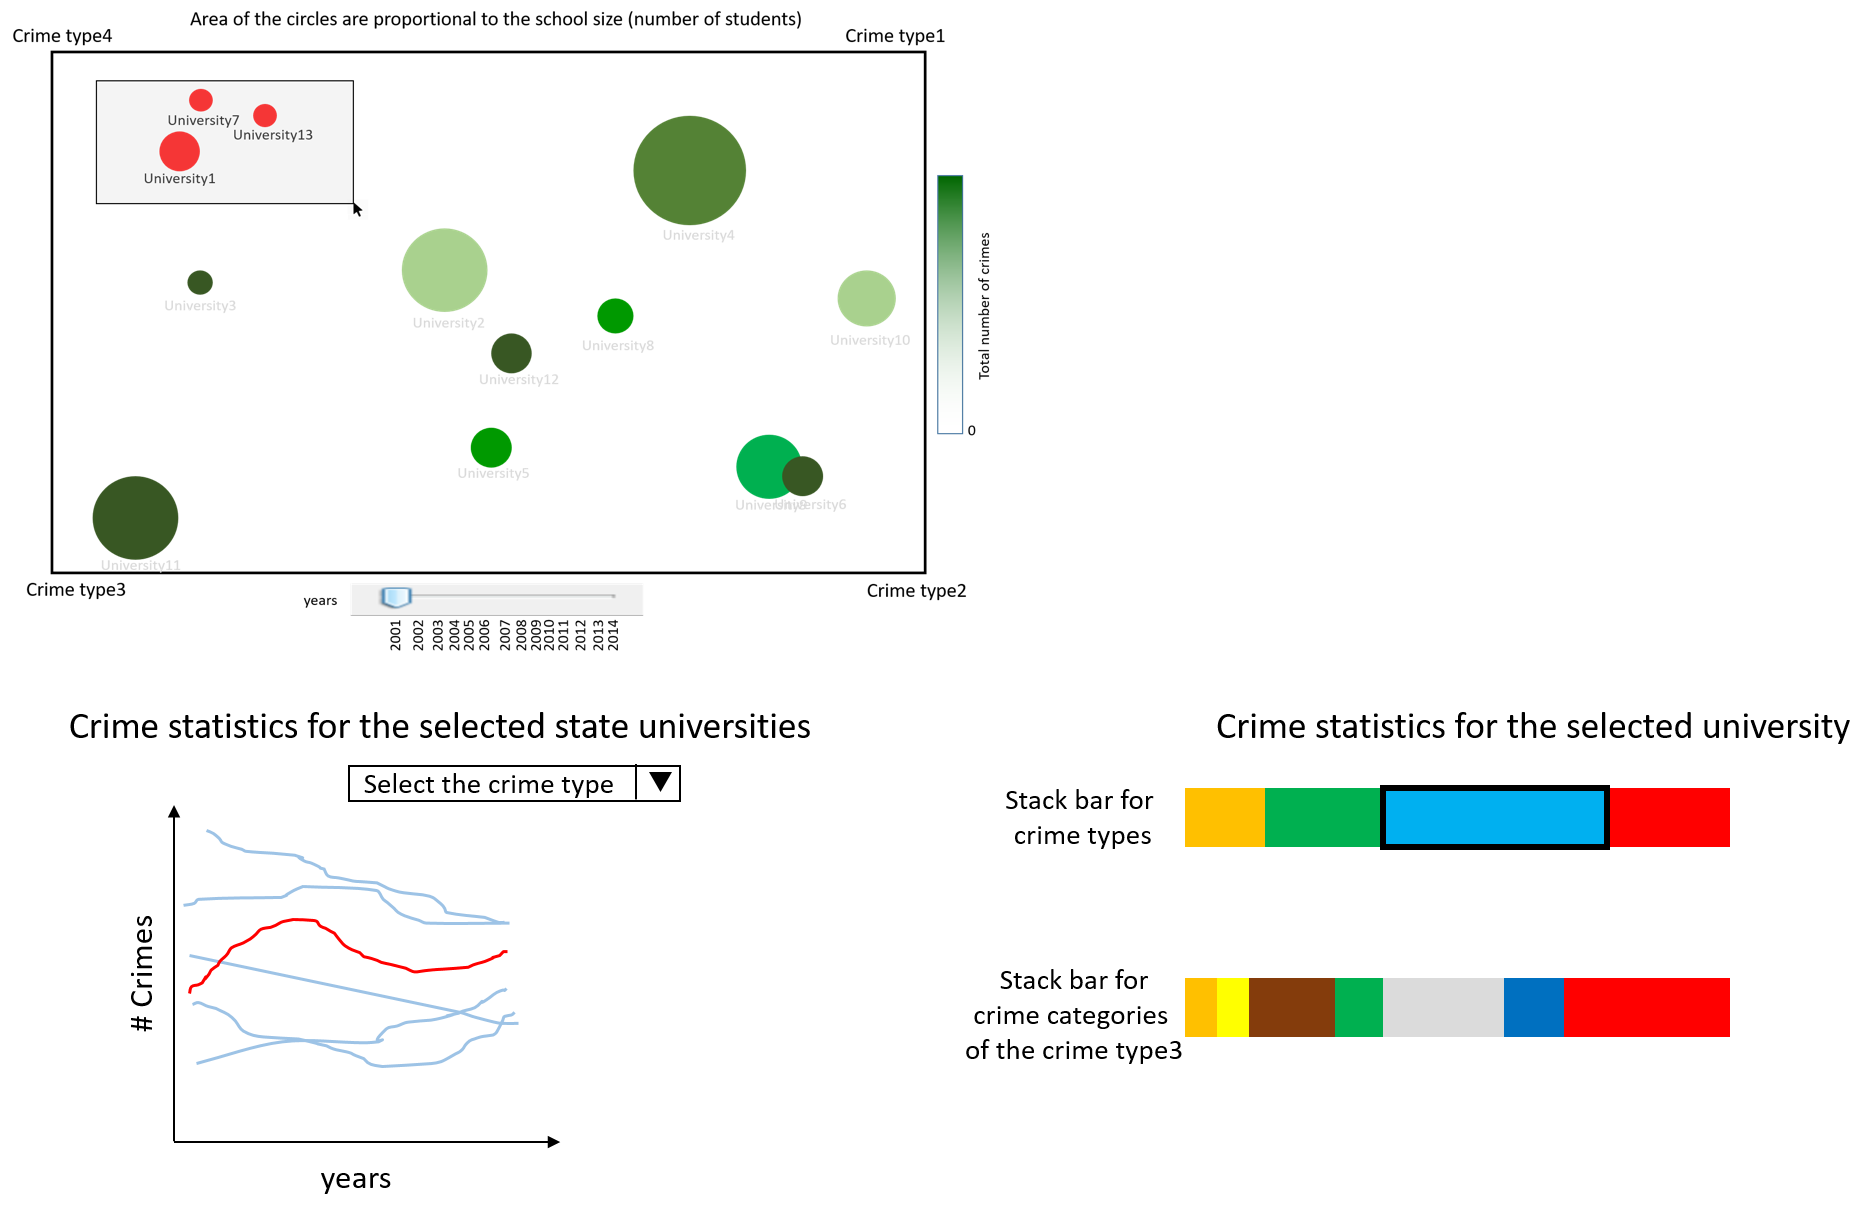
\includegraphics[width=6in]{prot2-3}           
\caption{}
\label{fig:p2-3}
\end{figure}


\noindent
\textbf{Our selected best design:}\\
We chose the first design and the third design as our best designs. In both of these designs we use a gradient colormap to qualitatively show a continuous attribute (number of crime per number of students). Then we use position for the most important data (cumber of crime in different categories). We have also used bar charts for separating categories and showing their amount. The stack barcharts are also used to show the percentage of each crime type or category, that uses length, the second best options. These designs, use color (second best choice for categorical attributes) to separates different categories since the spatial region is not available. The third design also uses spatial region to show crime types. 

But there is only one problem with the third design (\cref{fig:p2-overall}), which is there is a probability that the circles of two universities lay on top of each other and make it impossible to separate them. Because of this issue we decided to go with the first prototype (\cref{fig:p1-6}).
\\

\noindent
\textbf{Must-Have and Optional Features:}\\
We should be able to easily observe the crime statistics for different schools in each state and be able compare them. We should be able to see how different states are compared to each other in terms of crime statistics in their schools. Also, we should be able to see how these statistics have changed over the years.\\
As mentioned in the objectives, we'd like to combine this data set with other ones containing demographic information, GDP and such for different states and look for correlations between the crime rates and these attributes.

 

%----------------------------------------------------------------------------------------

\end{document}